\section{NOGWs in ground-based Lidar observations}
% NOGWs 
% Lidar observations in Q3D simulations are not useful / used y position 1 instead on npy/2!! --> use local 2D simulations for analysis of these plots (eventually conduct constant wind simulation again

% interpretation
Observations of GWs in the upper atmosphere are very limited. Besides satellite measurements (AIRS data) vertical time series from ground-based Lidar stations are the only measurements potentially available on a regular basis. The analysis of GWs in the these measurements is challenging and potential transient NOGW sources further complicate their interpretation. Therefore, section \ref{sec:lidOb-idealized} discusses vertical time series from a selection of idealized numerical simulations followed by a case study describing potential NOGWs from a propagating tropopause fold in CORAL measurements in section \ref{sec:lidOb-coral}.
 
\subsection{Lidar observations in idealized numerical simulations}
\label{sec:lidOb-idealized}
% The goal of the following analysis is 

Extend conclusions of \textcite{dornbrack_interpretation_2017}.



\begin{equation}
    \lambda_z = \frac{2*\Pi}{m} 
    \label{equ:lambdaz}
\end{equation}




%  Assuming \textcite{dornbrack_interpretation_2017}., the recorded period $T = 2π/ω$ can be used to obtain an estimate of the ground-based frequency ω. In such a case, the slope of the phase lines gives the vertical phase speed cPz = ± λz/T and the propagation directions of the wave phases and of the wave packet, respectively. Using an estimate of the background stratification N, the phase angle φ can be estimated from Equation (8) and k can be computed. Technically, the Equations (12) and (13) can now be employed to derive the components of the group velocity cgx and cgz from the known values of k, m, and φ. Summarizing the assumpti


show for constant wind and idealized stratospheric winter profile

In the thorough descripition of 


As usual, the vertical wavelength in the  be derived from the Lidar observation with

\begin{equation}
    \lambda_z = \frac{2*\Pi}{m} 
    \label{equ:lambdaz}
\end{equation}

\begin{equation}
    \lambda_z = \frac{2*\Pi}{m} 
    \label{equ:lambdaz}
\end{equation}


\begin{equation}
\begin{aligned}
    \frac{d \Vec{v}}{dt} = -G \Vec{\nabla} (\frac{p'}{\bar{\rho}}) +  \Vec{g} \frac{\theta'}{\bar{\theta}} - 2 \Vec{\Omega} \times (\Vec{v}-\Vec{v_e}) \\
    - \Tilde{\alpha} (\Vec{v}-\Vec{v_e}) \equiv R^{v},
    \label{equ:momEqu}
\end{aligned}
\end{equation}

Alternative interpretations:

- downward propagating wave / wave breaking - secondary wave - fish bone pattern

- transient wave signal due to a varying wind forcing (direction and speed) 


\begin{figure*}[]
    \centering
    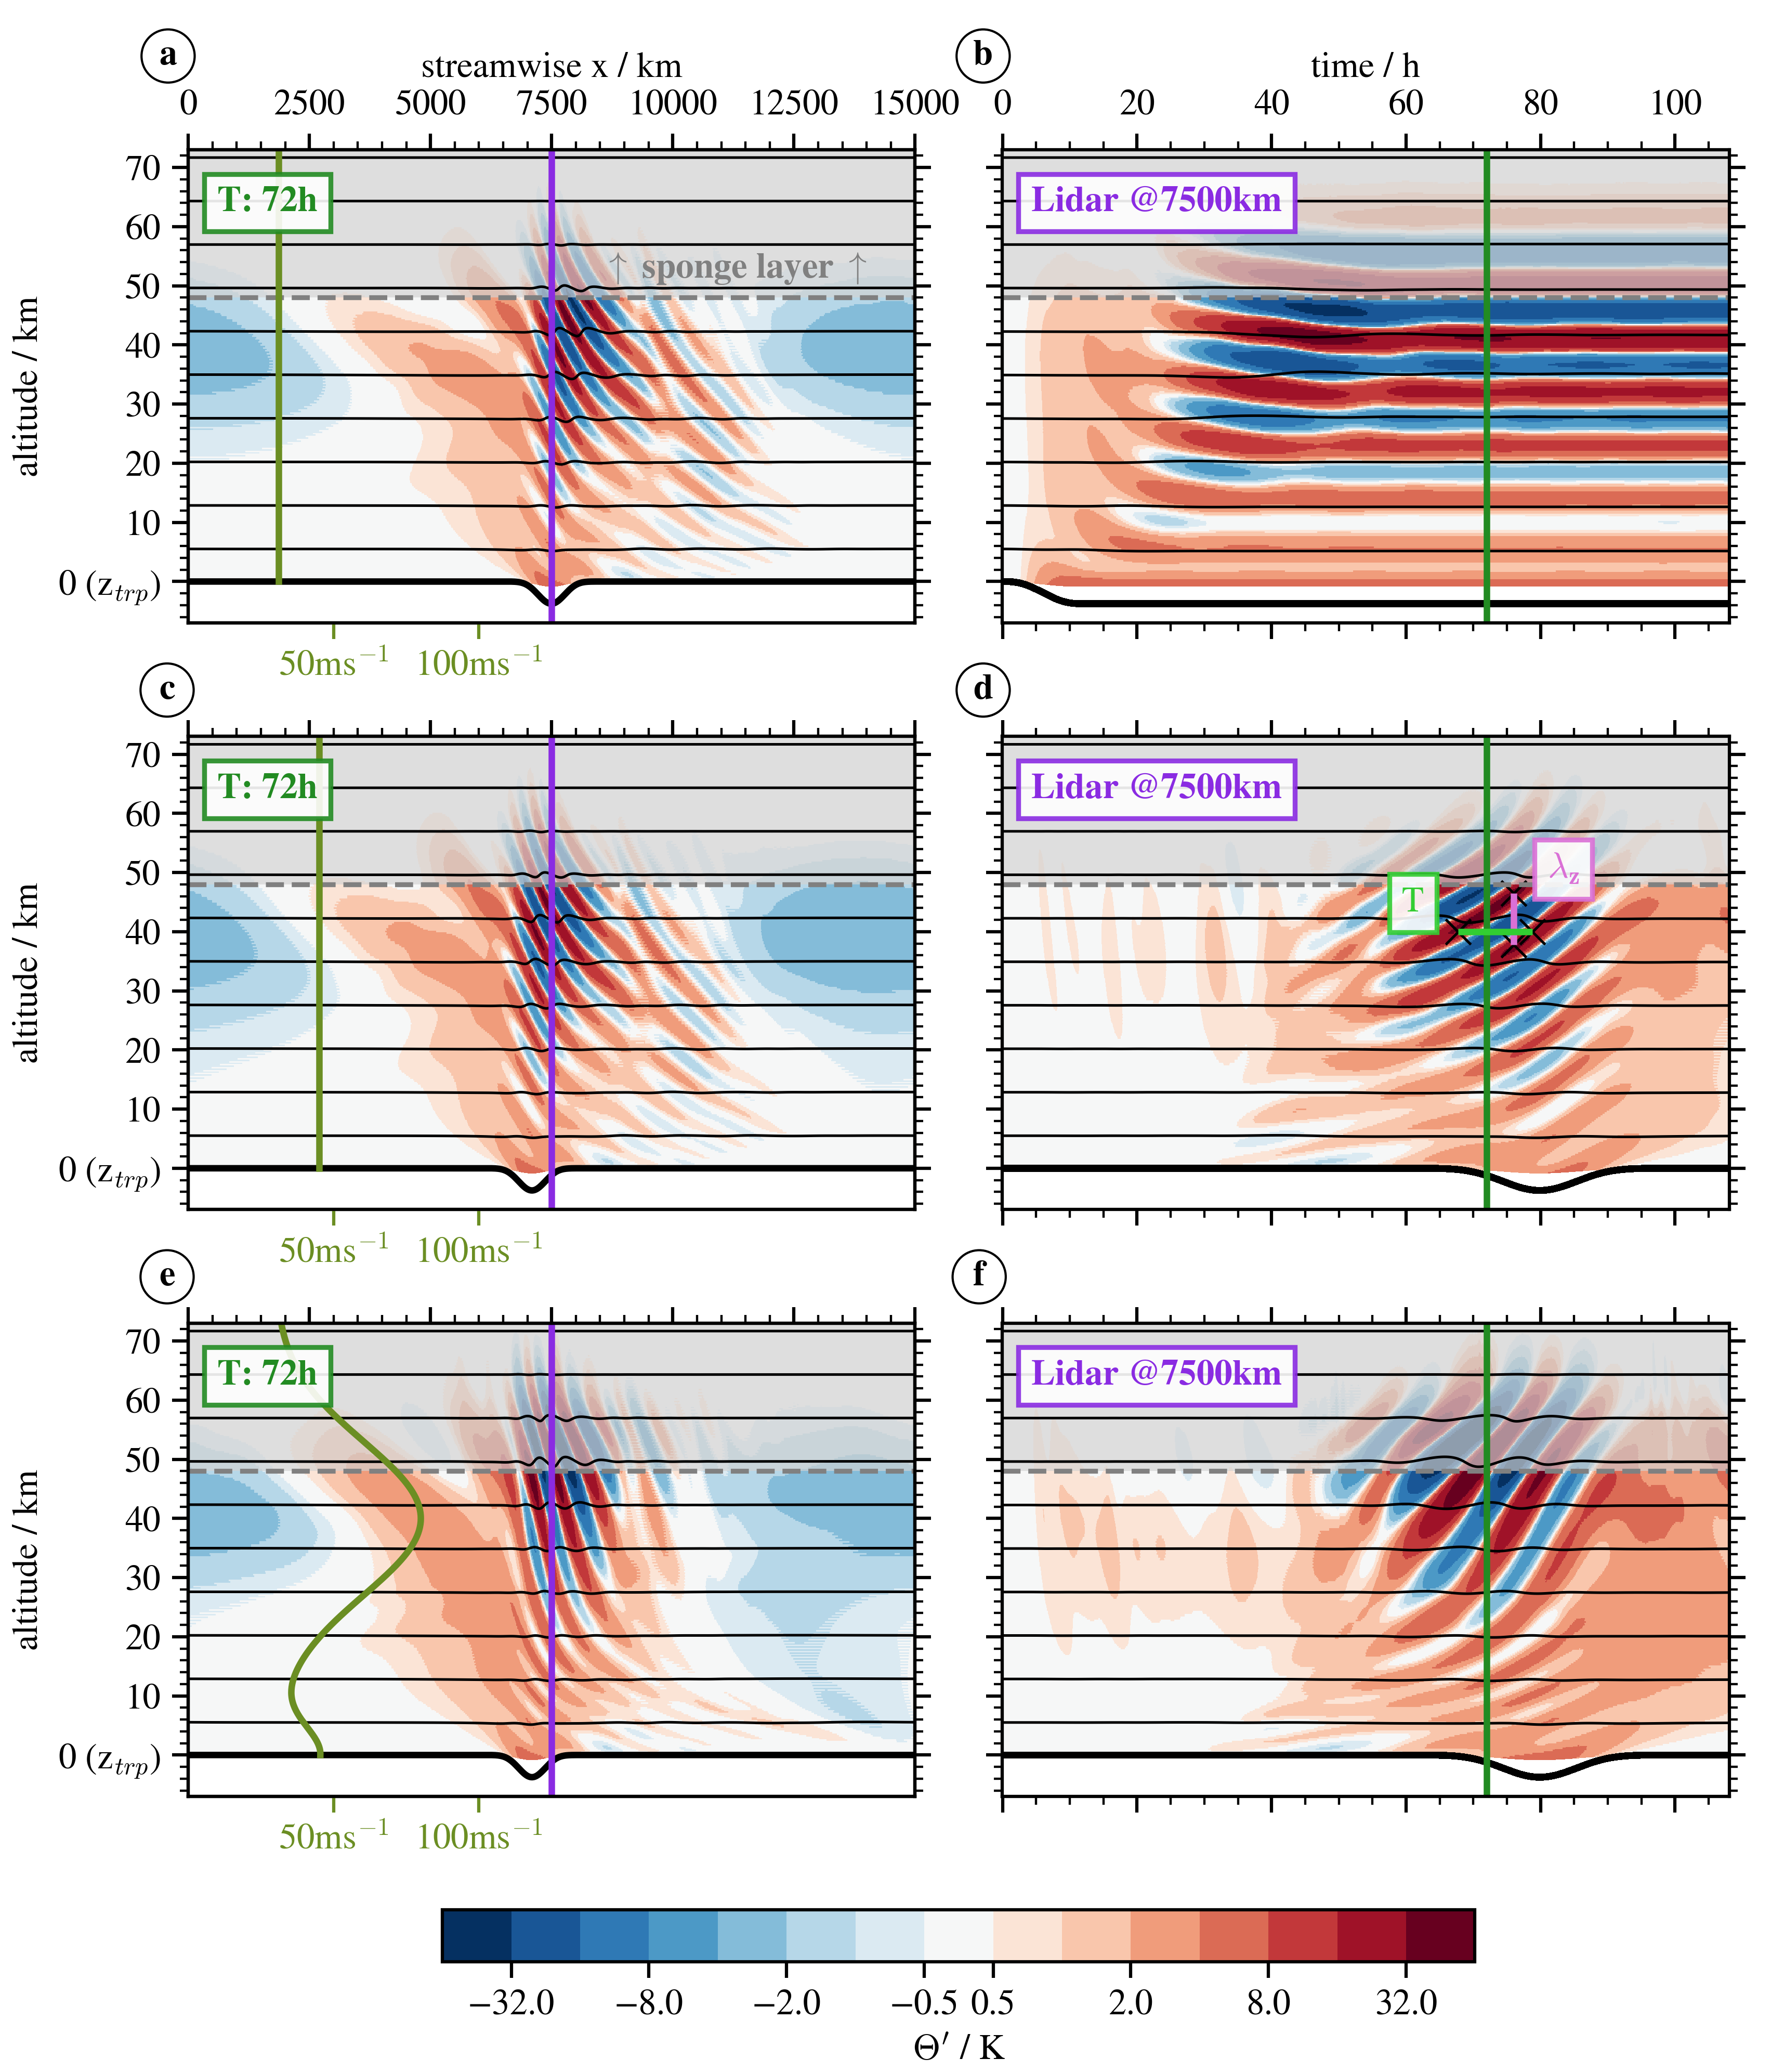
\includegraphics[width=0.99\textwidth]{figures_lidar/lidana_th.png}
    \caption{Vertical cross sections at 40km above the tropopause for five simulations with horizontal and meridional shear in a barotropic environment. Shown are $\theta$', $\lambda_x$ and $\lambda_y$ at 72h into the simulation. Dominant zonal and meridional wavelengths for each grid point are determined from wavelet analysis.}
    \label{fig:waveletAna_dudy}
\end{figure*}


\subsection{Coral observation of a transient GW source}
\label{sec:lidOb-coral}

This section provides a short introduction to an interesting Lidar observation of the Compact Autonomous Rayleigh Lidar (CORAL) at the southern tip of South America in Rio Grande, Argentina. 

Short description of CORAL...

\textcite{kaifler_compact_2021} provide a more extensive summary on CORAL's setup and observation, 

focus on observation from July 28th, 2018 showing upwards tilted lines of constant phase between 


